\documentclass[]{book}
\usepackage{lmodern}
\usepackage{amssymb,amsmath}
\usepackage{ifxetex,ifluatex}
\usepackage{fixltx2e} % provides \textsubscript
\ifnum 0\ifxetex 1\fi\ifluatex 1\fi=0 % if pdftex
  \usepackage[T1]{fontenc}
  \usepackage[utf8]{inputenc}
\else % if luatex or xelatex
  \ifxetex
    \usepackage{mathspec}
  \else
    \usepackage{fontspec}
  \fi
  \defaultfontfeatures{Ligatures=TeX,Scale=MatchLowercase}
\fi
% use upquote if available, for straight quotes in verbatim environments
\IfFileExists{upquote.sty}{\usepackage{upquote}}{}
% use microtype if available
\IfFileExists{microtype.sty}{%
\usepackage{microtype}
\UseMicrotypeSet[protrusion]{basicmath} % disable protrusion for tt fonts
}{}
\usepackage[margin=1in]{geometry}
\usepackage{hyperref}
\hypersetup{unicode=true,
            pdftitle={R Lab for Statistical Computing},
            pdfborder={0 0 0},
            breaklinks=true}
\urlstyle{same}  % don't use monospace font for urls
\usepackage{natbib}
\bibliographystyle{apalike}
\usepackage{color}
\usepackage{fancyvrb}
\newcommand{\VerbBar}{|}
\newcommand{\VERB}{\Verb[commandchars=\\\{\}]}
\DefineVerbatimEnvironment{Highlighting}{Verbatim}{commandchars=\\\{\}}
% Add ',fontsize=\small' for more characters per line
\usepackage{framed}
\definecolor{shadecolor}{RGB}{248,248,248}
\newenvironment{Shaded}{\begin{snugshade}}{\end{snugshade}}
\newcommand{\KeywordTok}[1]{\textcolor[rgb]{0.13,0.29,0.53}{\textbf{#1}}}
\newcommand{\DataTypeTok}[1]{\textcolor[rgb]{0.13,0.29,0.53}{#1}}
\newcommand{\DecValTok}[1]{\textcolor[rgb]{0.00,0.00,0.81}{#1}}
\newcommand{\BaseNTok}[1]{\textcolor[rgb]{0.00,0.00,0.81}{#1}}
\newcommand{\FloatTok}[1]{\textcolor[rgb]{0.00,0.00,0.81}{#1}}
\newcommand{\ConstantTok}[1]{\textcolor[rgb]{0.00,0.00,0.00}{#1}}
\newcommand{\CharTok}[1]{\textcolor[rgb]{0.31,0.60,0.02}{#1}}
\newcommand{\SpecialCharTok}[1]{\textcolor[rgb]{0.00,0.00,0.00}{#1}}
\newcommand{\StringTok}[1]{\textcolor[rgb]{0.31,0.60,0.02}{#1}}
\newcommand{\VerbatimStringTok}[1]{\textcolor[rgb]{0.31,0.60,0.02}{#1}}
\newcommand{\SpecialStringTok}[1]{\textcolor[rgb]{0.31,0.60,0.02}{#1}}
\newcommand{\ImportTok}[1]{#1}
\newcommand{\CommentTok}[1]{\textcolor[rgb]{0.56,0.35,0.01}{\textit{#1}}}
\newcommand{\DocumentationTok}[1]{\textcolor[rgb]{0.56,0.35,0.01}{\textbf{\textit{#1}}}}
\newcommand{\AnnotationTok}[1]{\textcolor[rgb]{0.56,0.35,0.01}{\textbf{\textit{#1}}}}
\newcommand{\CommentVarTok}[1]{\textcolor[rgb]{0.56,0.35,0.01}{\textbf{\textit{#1}}}}
\newcommand{\OtherTok}[1]{\textcolor[rgb]{0.56,0.35,0.01}{#1}}
\newcommand{\FunctionTok}[1]{\textcolor[rgb]{0.00,0.00,0.00}{#1}}
\newcommand{\VariableTok}[1]{\textcolor[rgb]{0.00,0.00,0.00}{#1}}
\newcommand{\ControlFlowTok}[1]{\textcolor[rgb]{0.13,0.29,0.53}{\textbf{#1}}}
\newcommand{\OperatorTok}[1]{\textcolor[rgb]{0.81,0.36,0.00}{\textbf{#1}}}
\newcommand{\BuiltInTok}[1]{#1}
\newcommand{\ExtensionTok}[1]{#1}
\newcommand{\PreprocessorTok}[1]{\textcolor[rgb]{0.56,0.35,0.01}{\textit{#1}}}
\newcommand{\AttributeTok}[1]{\textcolor[rgb]{0.77,0.63,0.00}{#1}}
\newcommand{\RegionMarkerTok}[1]{#1}
\newcommand{\InformationTok}[1]{\textcolor[rgb]{0.56,0.35,0.01}{\textbf{\textit{#1}}}}
\newcommand{\WarningTok}[1]{\textcolor[rgb]{0.56,0.35,0.01}{\textbf{\textit{#1}}}}
\newcommand{\AlertTok}[1]{\textcolor[rgb]{0.94,0.16,0.16}{#1}}
\newcommand{\ErrorTok}[1]{\textcolor[rgb]{0.64,0.00,0.00}{\textbf{#1}}}
\newcommand{\NormalTok}[1]{#1}
\usepackage{longtable,booktabs}
\usepackage{graphicx,grffile}
\makeatletter
\def\maxwidth{\ifdim\Gin@nat@width>\linewidth\linewidth\else\Gin@nat@width\fi}
\def\maxheight{\ifdim\Gin@nat@height>\textheight\textheight\else\Gin@nat@height\fi}
\makeatother
% Scale images if necessary, so that they will not overflow the page
% margins by default, and it is still possible to overwrite the defaults
% using explicit options in \includegraphics[width, height, ...]{}
\setkeys{Gin}{width=\maxwidth,height=\maxheight,keepaspectratio}
\IfFileExists{parskip.sty}{%
\usepackage{parskip}
}{% else
\setlength{\parindent}{0pt}
\setlength{\parskip}{6pt plus 2pt minus 1pt}
}
\setlength{\emergencystretch}{3em}  % prevent overfull lines
\providecommand{\tightlist}{%
  \setlength{\itemsep}{0pt}\setlength{\parskip}{0pt}}
\setcounter{secnumdepth}{5}
% Redefines (sub)paragraphs to behave more like sections
\ifx\paragraph\undefined\else
\let\oldparagraph\paragraph
\renewcommand{\paragraph}[1]{\oldparagraph{#1}\mbox{}}
\fi
\ifx\subparagraph\undefined\else
\let\oldsubparagraph\subparagraph
\renewcommand{\subparagraph}[1]{\oldsubparagraph{#1}\mbox{}}
\fi

%%% Use protect on footnotes to avoid problems with footnotes in titles
\let\rmarkdownfootnote\footnote%
\def\footnote{\protect\rmarkdownfootnote}

%%% Change title format to be more compact
\usepackage{titling}

% Create subtitle command for use in maketitle
\providecommand{\subtitle}[1]{
  \posttitle{
    \begin{center}\large#1\end{center}
    }
}

\setlength{\droptitle}{-2em}

  \title{R Lab for Statistical Computing}
    \pretitle{\vspace{\droptitle}\centering\huge}
  \posttitle{\par}
    \author{Young-geun Kim\\
Department of Statistics, SKKU\\
\href{mailto: dudrms33@g.skku.edu}{dudrms33@g.skku.edu}}
    \preauthor{\centering\large\emph}
  \postauthor{\par}
      \predate{\centering\large\emph}
  \postdate{\par}
    \date{2019-04-01}

\usepackage{booktabs}
\usepackage{float}
\usepackage{pdfpages}

\let\oldmaketitle\maketitle
\AtBeginDocument{\let\maketitle\relax}

\usepackage{amsthm}
\newtheorem{theorem}{Theorem}[chapter]
\newtheorem{lemma}{Lemma}[chapter]
\newtheorem{corollary}{Corollary}[chapter]
\newtheorem{proposition}{Proposition}[chapter]
\newtheorem{conjecture}{Conjecture}[chapter]
\theoremstyle{definition}
\newtheorem{definition}{Definition}[chapter]
\theoremstyle{definition}
\newtheorem{example}{Example}[chapter]
\theoremstyle{definition}
\newtheorem{exercise}{Exercise}[chapter]
\theoremstyle{remark}
\newtheorem*{remark}{Remark}
\newtheorem*{solution}{Solution}
\let\BeginKnitrBlock\begin \let\EndKnitrBlock\end
\begin{document}
\maketitle

\begin{titlepage}
  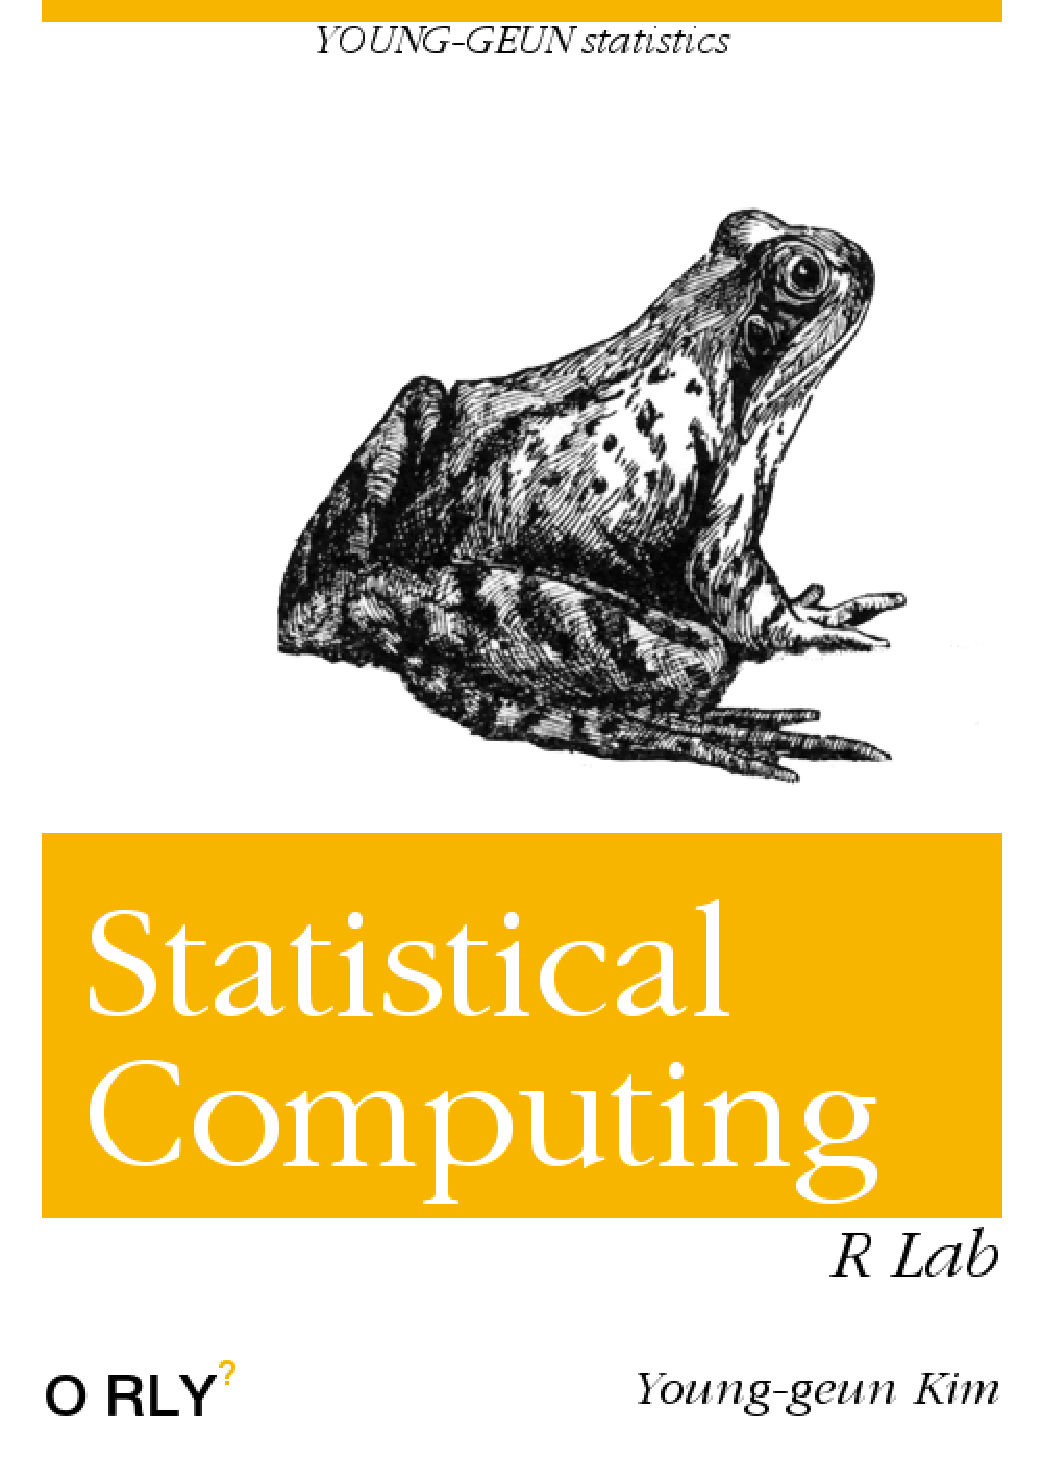
\includepdf{cover.pdf}
\end{titlepage}

\let\maketitle\oldmaketitle
\maketitle

{
\setcounter{tocdepth}{1}
\tableofcontents
}
\chapter*{Welcome}\label{welcome}
\addcontentsline{toc}{chapter}{Welcome}

 Statistical computing mainly treats useful simulation methods.

\section*{Statistical Computing}\label{statistical-computing}
\addcontentsline{toc}{section}{Statistical Computing}

We first look at \emph{random generation} methods. Lots of simulation
methods are built based on this random numbers.

\subsection*{Sampling from a fininte
population}\label{sampling-from-a-fininte-population}
\addcontentsline{toc}{subsection}{Sampling from a fininte population}

Generating random numbers is like sampling. From finite population, we
can sample data with or without replacement. For example of sampling
with replacement, we toss coins 10 times.

\begin{Shaded}
\begin{Highlighting}[]
\KeywordTok{sample}\NormalTok{(}\DecValTok{0}\OperatorTok{:}\DecValTok{1}\NormalTok{, }\DataTypeTok{size =} \DecValTok{10}\NormalTok{, }\DataTypeTok{replace =} \OtherTok{TRUE}\NormalTok{)}
\end{Highlighting}
\end{Shaded}

\begin{verbatim}
 [1] 1 0 0 1 0 1 1 0 1 1
\end{verbatim}

Sampling without replacement: Choose some lottery numbers which consist
of 1 to 100.

\begin{Shaded}
\begin{Highlighting}[]
\KeywordTok{sample}\NormalTok{(}\DecValTok{1}\OperatorTok{:}\DecValTok{100}\NormalTok{, }\DataTypeTok{size =} \DecValTok{6}\NormalTok{, }\DataTypeTok{replace =} \OtherTok{FALSE}\NormalTok{)}
\end{Highlighting}
\end{Shaded}

\begin{verbatim}
[1] 61 83 50 74 34 35
\end{verbatim}

\subsection*{Random generators of common probability
distributions}\label{random-generators-of-common-probability-distributions}
\addcontentsline{toc}{subsection}{Random generators of common
probability distributions}

\texttt{R} provides some functions which generate random numbers
following famous distributions. Although we will learn some skills
generating these numbers in basis levels, these functions do the same
thing more elegantly.

\begin{Shaded}
\begin{Highlighting}[]
\KeywordTok{gg_curve}\NormalTok{(dbeta, }\DataTypeTok{from =} \DecValTok{0}\NormalTok{, }\DataTypeTok{to =} \DecValTok{1}\NormalTok{, }\DataTypeTok{args =} \KeywordTok{list}\NormalTok{(}\DataTypeTok{shape1 =} \DecValTok{3}\NormalTok{, }\DataTypeTok{shape2 =} \DecValTok{2}\NormalTok{)) }\OperatorTok{+}
\StringTok{  }\KeywordTok{geom_histogram}\NormalTok{(}
    \DataTypeTok{data =} \KeywordTok{tibble}\NormalTok{(}
      \DataTypeTok{rand =} \KeywordTok{rbeta}\NormalTok{(}\DecValTok{1000}\NormalTok{, }\DecValTok{3}\NormalTok{, }\DecValTok{2}\NormalTok{),}
      \DataTypeTok{idx =} \KeywordTok{seq}\NormalTok{(}\DecValTok{0}\NormalTok{, }\DecValTok{1}\NormalTok{, }\DataTypeTok{length.out =} \DecValTok{1000}\NormalTok{)}
\NormalTok{    ),}
    \KeywordTok{aes}\NormalTok{(}\DataTypeTok{x =}\NormalTok{ rand, }\DataTypeTok{y =}\NormalTok{ ..density..),}
    \DataTypeTok{position =} \StringTok{"identity"}\NormalTok{,}
    \DataTypeTok{bins =} \DecValTok{30}\NormalTok{,}
    \DataTypeTok{alpha =}\NormalTok{ .}\DecValTok{45}\NormalTok{,}
    \DataTypeTok{fill =} \KeywordTok{gg_hcl}\NormalTok{(}\DecValTok{1}\NormalTok{)}
\NormalTok{  )}
\end{Highlighting}
\end{Shaded}

\begin{figure}[H]

{\centering 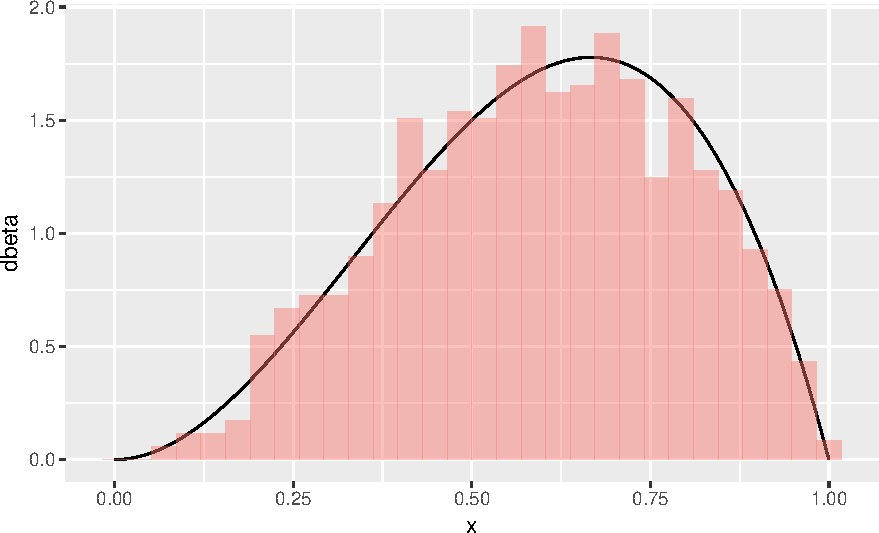
\includegraphics[width=0.7\linewidth]{statistical-computing_files/figure-latex/dbrb-1} 

}

\caption{Beta(3,2) random numbers}\label{fig:dbrb}
\end{figure}

Figure \ref{fig:dbrb} shows that \texttt{rbeta()} function generate
random numbers very well. Histogram is of the random number, and the
curve is the true beta distribution.

\chapter{Methods for Generating Random Variables}\label{rvar}

\section{Introduction}\label{introduction}

Most of the methods so-called \emph{computational statistics} requires
generation of random variables from specified probability distribution.
In hand, we can spin wheels, roll a dice, or shuffle cards. The results
are chosen randomly. However, we want the same things with computer.
Here, \texttt{r}. As we know, computer cannot generate complete uniform
random numbers. Instead, we generate \textbf{pseudo-random} numbers.

\section{Pseudo-random Numbers}\label{pseudo-random-numbers}

\BeginKnitrBlock{definition}[Pseudo-random numbers]
\protect\hypertarget{def:unnamed-chunk-5}{}{\label{def:unnamed-chunk-5}
\iffalse (Pseudo-random numbers) \fi{} }Sequence of values generated
deterministically which have all the appearances of being independent
\(unif(0, 1)\) random variables, i.e.

\[x_1, x_2, \ldots, x_n \stackrel{iid}{\sim} unif(0, 1)\]
\EndKnitrBlock{definition}

\begin{itemize}
\tightlist
\item
  behave \emph{as if} following \(unif(0, 1)\)
\item
  typically generated from an \emph{initial seed}
\end{itemize}

\subsection{Linear congruential
generator}\label{linear-congruential-generator}

Let \(x_0, x_1, \ldots \in \mathbb{Z}_{+}\).

\begin{enumerate}
\def\labelenumi{\arabic{enumi}.}
\tightlist
\item
  Set \(x_0\) as initial seed.
\item
  Generate \(x_n, n = 1, 2, \ldots\) recursively:

  \begin{enumerate}
  \def\labelenumii{\alph{enumii}.}
  \tightlist
  \item
    \(x_n = (a x_{n - 1} + c) \mod m\)
  \item
    where \(a, c \in \mathbb{Z}_{+}, m: \text{modulus}\)
  \end{enumerate}
\item
  Compute \(u_n = \frac{x_n}{m} \in (0, 1)\)
\end{enumerate}

Then \(u_1, u_2, \ldots \sim unif(0, 1)\)

\begin{Shaded}
\begin{Highlighting}[]
\NormalTok{lcg <-}\StringTok{ }\ControlFlowTok{function}\NormalTok{(n, seed, a, b, m) \{}
\NormalTok{  x <-}\StringTok{ }\KeywordTok{rep}\NormalTok{(seed, n }\OperatorTok{+}\StringTok{ }\DecValTok{1}\NormalTok{)}
  \ControlFlowTok{for}\NormalTok{ (i }\ControlFlowTok{in} \DecValTok{1}\OperatorTok{:}\NormalTok{n) \{}
\NormalTok{    x[i }\OperatorTok{+}\StringTok{ }\DecValTok{1}\NormalTok{] <-}\StringTok{ }\NormalTok{(a }\OperatorTok{*}\StringTok{ }\NormalTok{x[i] }\OperatorTok{+}\StringTok{ }\NormalTok{b) }\OperatorTok\StringTok{ }\NormalTok{m}
\NormalTok{  \}}
\NormalTok{  x[}\OperatorTok{-}\DecValTok{1}\NormalTok{] }\OperatorTok{/}\StringTok{ }\NormalTok{m}
\NormalTok{\}}
\end{Highlighting}
\end{Shaded}

\begin{Shaded}
\begin{Highlighting}[]
\KeywordTok{tibble}\NormalTok{(}
  \DataTypeTok{x =} \KeywordTok{lcg}\NormalTok{(}\DecValTok{1000}\NormalTok{, }\DecValTok{0}\NormalTok{, }\DecValTok{1664525}\NormalTok{, }\DecValTok{1013904223}\NormalTok{, }\DecValTok{2}\OperatorTok{^}\DecValTok{32}\NormalTok{)}
\NormalTok{) }\OperatorTok\StringTok{ }
\StringTok{  }\KeywordTok{ggplot}\NormalTok{(}\KeywordTok{aes}\NormalTok{(}\DataTypeTok{x =}\NormalTok{ x)) }\OperatorTok{+}
\StringTok{  }\KeywordTok{geom_histogram}\NormalTok{(}\KeywordTok{aes}\NormalTok{(}\DataTypeTok{y =}\NormalTok{ ..density..), }\DataTypeTok{bins =} \DecValTok{30}\NormalTok{, }\DataTypeTok{col =} \KeywordTok{gg_hcl}\NormalTok{(}\DecValTok{1}\NormalTok{))}
\end{Highlighting}
\end{Shaded}

\begin{center}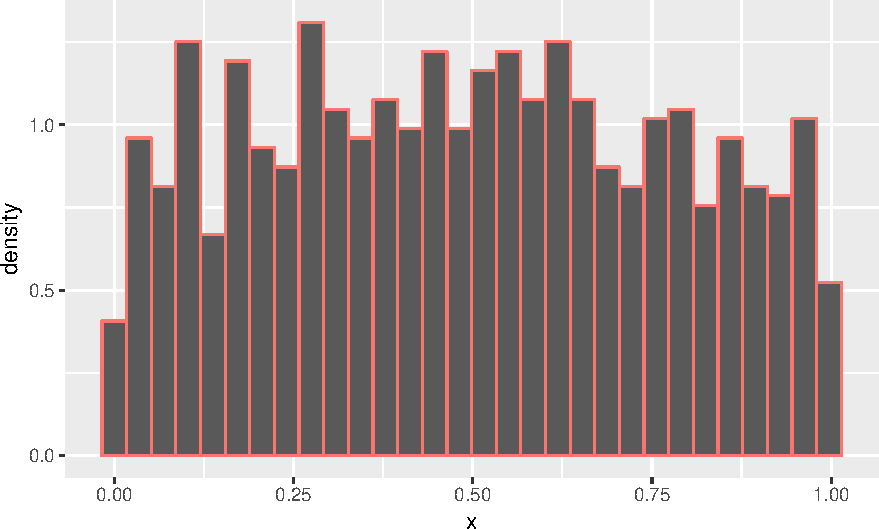
\includegraphics[width=0.7\linewidth]{statistical-computing_files/figure-latex/unnamed-chunk-7-1} \end{center}

\subsection{Multiplicative congruential
generator}\label{multiplicative-congruential-generator}

As we can expect from its name, this is congruential generator with
\(c = 0\).

\begin{enumerate}
\def\labelenumi{\arabic{enumi}.}
\tightlist
\item
  Set \(x_0\) as initial seed.
\item
  Generate \(x_n, n = 1, 2, \ldots\) recursively:

  \begin{enumerate}
  \def\labelenumii{\alph{enumii}.}
  \tightlist
  \item
    \(x_n = a x_{n - 1} \mod m\)
  \item
    where \(a \in \mathbb{Z}_{+}, m: \text{modulus}\)
  \end{enumerate}
\item
  Compute \(u_n = \frac{x_n}{m} \in (0, 1)\)
\end{enumerate}

Then \(u_1, u_2, \ldots \sim unif(0, 1)\)

We just set \texttt{b\ =\ 0} in our \texttt{lcg()} function. The
\textbf{seed must not be zero}.

\begin{Shaded}
\begin{Highlighting}[]
\KeywordTok{tibble}\NormalTok{(}
  \DataTypeTok{x =} \KeywordTok{lcg}\NormalTok{(}\DecValTok{1000}\NormalTok{, }\DecValTok{5}\NormalTok{, }\DecValTok{1664525}\NormalTok{, }\DecValTok{0}\NormalTok{, }\DecValTok{2}\OperatorTok{^}\DecValTok{32}\NormalTok{)}
\NormalTok{) }\OperatorTok\StringTok{ }
\StringTok{  }\KeywordTok{ggplot}\NormalTok{(}\KeywordTok{aes}\NormalTok{(}\DataTypeTok{x =}\NormalTok{ x)) }\OperatorTok{+}
\StringTok{  }\KeywordTok{geom_histogram}\NormalTok{(}\KeywordTok{aes}\NormalTok{(}\DataTypeTok{y =}\NormalTok{ ..density..), }\DataTypeTok{bins =} \DecValTok{30}\NormalTok{, }\DataTypeTok{col =} \KeywordTok{gg_hcl}\NormalTok{(}\DecValTok{1}\NormalTok{))}
\end{Highlighting}
\end{Shaded}

\begin{center}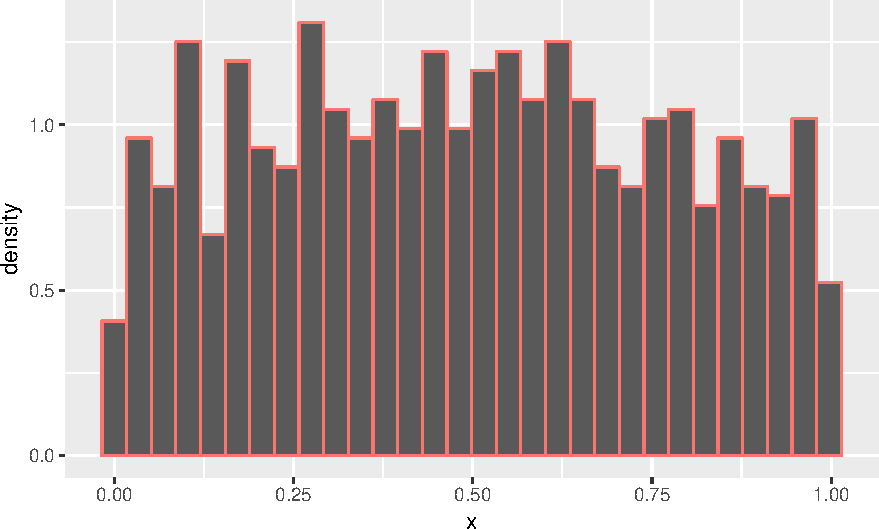
\includegraphics[width=0.7\linewidth]{statistical-computing_files/figure-latex/unnamed-chunk-8-1} \end{center}

\subsection{Cycle}\label{cycle}

Generate LCG \(n = 32\) with \(a = 1\), \(c = 1\), and \(m = 16\) from
the seed \(x_0 = 0\).

\begin{Shaded}
\begin{Highlighting}[]
\KeywordTok{lcg}\NormalTok{(}\DecValTok{32}\NormalTok{, }\DecValTok{0}\NormalTok{, }\DecValTok{1}\NormalTok{, }\DecValTok{1}\NormalTok{, }\DecValTok{16}\NormalTok{)}
\end{Highlighting}
\end{Shaded}

\begin{verbatim}
 [1] 0.0625 0.1250 0.1875 0.2500 0.3125 0.3750 0.4375 0.5000 0.5625 0.6250
[11] 0.6875 0.7500 0.8125 0.8750 0.9375 0.0000 0.0625 0.1250 0.1875 0.2500
[21] 0.3125 0.3750 0.4375 0.5000 0.5625 0.6250 0.6875 0.7500 0.8125 0.8750
[31] 0.9375 0.0000
\end{verbatim}

Observe that we have the cycle after \(m\)-th number. Against this
problem, we give different seed from every \((im + 1)\)th random number.

\section{The Inverse Transform
Method}\label{the-inverse-transform-method}

\BeginKnitrBlock{definition}[Inverse of CDF]
\protect\hypertarget{def:icdf}{}{\label{def:icdf} \iffalse (Inverse of CDF)
\fi{} }Since some cdf \(F_X\) is not strictly increasing, we difine
\(F_X^{-1}(y)\) for \(0 < y < 1\) by

\[F_{X}^{-1}(y) := inf \{ x : F_X(x) \ge y \}\]
\EndKnitrBlock{definition}

Using this definition, we can get the following theorem.

\BeginKnitrBlock{theorem}[Probability Integral Transformation]
\protect\hypertarget{thm:probint}{}{\label{thm:probint}
\iffalse (Probability Integral Transformation) \fi{} }If \(X\) is a
continuous random variable with cdf \(F_(x)\), then
\[U \equiv F_X(X) \sim unif(0, 1)\]
\EndKnitrBlock{theorem}

\BeginKnitrBlock{proof}[Probability Integral Transformation]
\iffalse{} {Proof (Probability Integral Transformation). } \fi{}Let
\(U \sim unif(0, 1)\). Then

\begin{equation*}
  \begin{split}
    P(F_X^{-1}(U) \le x) & = P(\inf\{t : F_X(t) = U \} \le x) \\
    & = P(U \le F_X(x)) \\
    & = F_U(F_X(x)) \\
    & = F_X(x)
  \end{split}
\end{equation*}
\EndKnitrBlock{proof}

Thus, to generate \(n\) random variables \(\sim F_X\),

\begin{enumerate}
\def\labelenumi{\arabic{enumi}.}
\tightlist
\item
  form of \(F_X^{-1}(u)\)
\item
  For each \(i = 1, 2, \ldots, n\):

  \begin{enumerate}
  \def\labelenumii{\alph{enumii}.}
  \tightlist
  \item
    Generate \(u_i \sim unif(0, 1)\)
  \item
    \(x_i = F_X^{-1}(u_i)\)
  \end{enumerate}
\end{enumerate}

Collect \(x_1, x_2, \ldots, x_n \stackrel{iid}{\sim} F_X\).

\subsection{Continuous case}\label{continuous-case}

Denote that the \emph{probability integral transformation} holds for a
continuous variable. When generating continuous random variable,
applying above algorithm might work.

\BeginKnitrBlock{example}[Exponential distribution]
\protect\hypertarget{exm:expon}{}{\label{exm:expon} \iffalse (Exponential
distribution) \fi{} }If \(X \sim Exp(\lambda)\), then
\(F_X(x) = 1 - e^{-\lambda x}\). We can derive the inverse function of
cdf \[F_X^{-1}(u) = \frac{1}{\lambda}\ln(1 - u)\]
\EndKnitrBlock{example}

Note that

\[U \sim unif(0, 1) \Leftrightarrow 1 - U \sim unif(0,1 )\]

Then we just can use \(U\) instead of \(1 - U\).

\begin{Shaded}
\begin{Highlighting}[]
\NormalTok{inv_exp <-}\StringTok{ }\ControlFlowTok{function}\NormalTok{(n, lambda) \{}
  \OperatorTok{-}\KeywordTok{log}\NormalTok{(}\KeywordTok{runif}\NormalTok{(n)) }\OperatorTok{/}\StringTok{ }\NormalTok{lambda}
\NormalTok{\}}
\end{Highlighting}
\end{Shaded}

If we generate \(x_1, \ldots, x_{500} \sim Exp(\lambda = 1)\),

\begin{Shaded}
\begin{Highlighting}[]
\KeywordTok{gg_curve}\NormalTok{(dexp, }\DataTypeTok{from =} \DecValTok{0}\NormalTok{, }\DataTypeTok{to =} \DecValTok{10}\NormalTok{) }\OperatorTok{+}
\StringTok{  }\KeywordTok{geom_histogram}\NormalTok{(}
    \DataTypeTok{data =} \KeywordTok{tibble}\NormalTok{(}\DataTypeTok{x =} \KeywordTok{inv_exp}\NormalTok{(}\DecValTok{500}\NormalTok{, }\DataTypeTok{lambda =} \DecValTok{1}\NormalTok{)),}
    \KeywordTok{aes}\NormalTok{(}\DataTypeTok{x =}\NormalTok{ x, }\DataTypeTok{y =}\NormalTok{ ..density..),}
    \DataTypeTok{bins =} \DecValTok{30}\NormalTok{,}
    \DataTypeTok{fill =} \KeywordTok{gg_hcl}\NormalTok{(}\DecValTok{1}\NormalTok{),}
    \DataTypeTok{alpha =}\NormalTok{ .}\DecValTok{5}
\NormalTok{  )}
\end{Highlighting}
\end{Shaded}

\begin{figure}[H]

{\centering 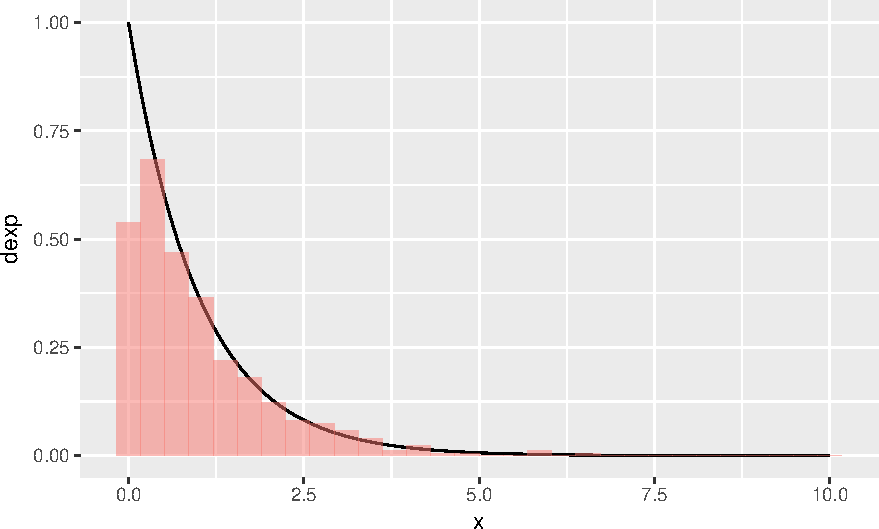
\includegraphics[width=0.7\linewidth]{statistical-computing_files/figure-latex/cdfexp-1} 

}

\caption{Inverse Transformation: Exp(1)}\label{fig:cdfexp}
\end{figure}

\subsection{Discrete case}\label{discrete-case}

\begin{enumerate}
\def\labelenumi{\arabic{enumi}.}
\tightlist
\item
  For each \(i = 1, 2, \ldots, n\):

  \begin{enumerate}
  \def\labelenumii{\alph{enumii}.}
  \tightlist
  \item
    Generate \(u_i \sim unif(0, 1)\)
  \item
    Take \(x_i\) s.t. \(F_X(x_{i - 1}) < U \le F_X(x_i)\)
  \end{enumerate}
\end{enumerate}

Collect \(x_1, x_2, \ldots, x_n \sim F_X\).

\begin{Shaded}
\begin{Highlighting}[]
\NormalTok{pmf <-}
\StringTok{  }\KeywordTok{tibble}\NormalTok{(}
    \DataTypeTok{x =} \DecValTok{0}\OperatorTok{:}\DecValTok{4}\NormalTok{,}
    \DataTypeTok{p =} \KeywordTok{c}\NormalTok{(.}\DecValTok{1}\NormalTok{, .}\DecValTok{2}\NormalTok{, .}\DecValTok{2}\NormalTok{, .}\DecValTok{2}\NormalTok{, .}\DecValTok{3}\NormalTok{)}
\NormalTok{  )}
\end{Highlighting}
\end{Shaded}

\begin{longtable}[]{@{}lrrrrr@{}}
\caption{\label{tab:exdis}Example of a Discrete Random
Variable}\tabularnewline
\toprule
x & 0.0 & 1.0 & 2.0 & 3.0 & 4.0\tabularnewline
p & 0.1 & 0.2 & 0.2 & 0.2 & 0.3\tabularnewline
\bottomrule
\end{longtable}

\BeginKnitrBlock{example}[Discrete Random Variable]
\protect\hypertarget{exm:dismass}{}{\label{exm:dismass} \iffalse (Discrete
Random Variable) \fi{} }Consider a discrete random variable \(X\) with a
mass function as in Table \ref{tab:exdis}.
\EndKnitrBlock{example}

i.e.

\begin{Shaded}
\begin{Highlighting}[]
\NormalTok{pmf }\OperatorTok\StringTok{ }
\StringTok{  }\KeywordTok{ggplot}\NormalTok{() }\OperatorTok{+}
\StringTok{  }\KeywordTok{geom_segment}\NormalTok{(}\KeywordTok{aes}\NormalTok{(}\DataTypeTok{x =}\NormalTok{ x, }\DataTypeTok{y =} \DecValTok{0}\NormalTok{, }\DataTypeTok{xend =}\NormalTok{ x, }\DataTypeTok{yend =}\NormalTok{ p)) }\OperatorTok{+}
\StringTok{  }\KeywordTok{ylab}\NormalTok{(}\KeywordTok{expression}\NormalTok{(}\KeywordTok{p}\NormalTok{(x)))}
\end{Highlighting}
\end{Shaded}

\begin{figure}[H]

{\centering 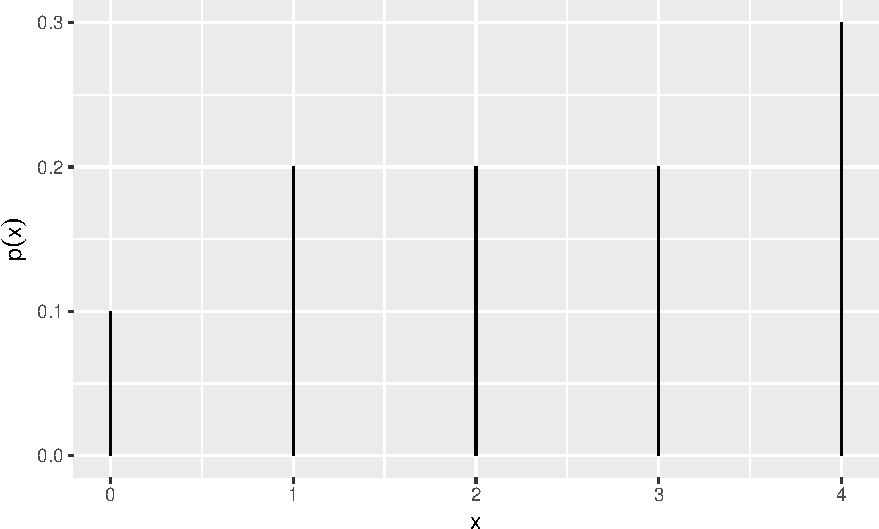
\includegraphics[width=0.7\linewidth]{statistical-computing_files/figure-latex/massfun-1} 

}

\caption{Probability Mass Function}\label{fig:massfun}
\end{figure}

Then we have the cdf

\begin{Shaded}
\begin{Highlighting}[]
\NormalTok{pmf }\OperatorTok\StringTok{ }
\StringTok{  }\KeywordTok{mutate}\NormalTok{(}
    \DataTypeTok{fx =} \KeywordTok{cumsum}\NormalTok{(p),}
    \DataTypeTok{x_end =} \KeywordTok{lead}\NormalTok{(x, }\DataTypeTok{default =} \DecValTok{5}\NormalTok{),}
    \DataTypeTok{u =}\NormalTok{ fx,}
    \DataTypeTok{u =} \KeywordTok{ifelse}\NormalTok{(u }\OperatorTok{==}\StringTok{ }\NormalTok{.}\DecValTok{5}\NormalTok{, .}\DecValTok{6}\NormalTok{, u),}
    \DataTypeTok{fx1 =} \KeywordTok{lead}\NormalTok{(fx, }\DataTypeTok{default =} \DecValTok{1}\NormalTok{),}
    \DataTypeTok{rand =}\NormalTok{ u }\OperatorTok{>}\StringTok{ }\NormalTok{fx }\OperatorTok{&}\StringTok{ }\NormalTok{u }\OperatorTok{<=}\StringTok{ }\NormalTok{fx1}
\NormalTok{  ) }\OperatorTok\StringTok{ }
\StringTok{  }\KeywordTok{ggplot}\NormalTok{() }\OperatorTok{+}
\StringTok{  }\KeywordTok{geom_segment}\NormalTok{(}\KeywordTok{aes}\NormalTok{(}\DataTypeTok{x =}\NormalTok{ x, }\DataTypeTok{y =}\NormalTok{ fx, }\DataTypeTok{xend =}\NormalTok{ x_end, }\DataTypeTok{yend =}\NormalTok{ fx)) }\OperatorTok{+}
\StringTok{  }\KeywordTok{ylab}\NormalTok{(}\KeywordTok{expression}\NormalTok{(}\KeywordTok{F}\NormalTok{(x))) }\OperatorTok{+}
\StringTok{  }\KeywordTok{geom_segment}\NormalTok{(}
    \KeywordTok{aes}\NormalTok{(}\DataTypeTok{x =} \DecValTok{0}\NormalTok{, }\DataTypeTok{y =}\NormalTok{ u, }\DataTypeTok{xend =}\NormalTok{ x_end, }\DataTypeTok{yend =}\NormalTok{ u, }\DataTypeTok{colour =}\NormalTok{ rand),}
    \DataTypeTok{linetype =} \StringTok{"dashed"}\NormalTok{,}
    \DataTypeTok{arrow =} \KeywordTok{arrow}\NormalTok{(}\DataTypeTok{length =} \KeywordTok{unit}\NormalTok{(.}\DecValTok{5}\NormalTok{, }\StringTok{"cm"}\NormalTok{)),}
    \DataTypeTok{show.legend =} \OtherTok{FALSE}
\NormalTok{  ) }\OperatorTok{+}
\StringTok{  }\KeywordTok{geom_segment}\NormalTok{(}
    \KeywordTok{aes}\NormalTok{(}\DataTypeTok{x =}\NormalTok{ x_end, }\DataTypeTok{y =}\NormalTok{ u, }\DataTypeTok{xend =}\NormalTok{ x_end, }\DataTypeTok{yend =} \DecValTok{0}\NormalTok{, }\DataTypeTok{colour =}\NormalTok{ rand),}
    \DataTypeTok{linetype =} \StringTok{"dashed"}\NormalTok{,}
    \DataTypeTok{arrow =} \KeywordTok{arrow}\NormalTok{(}\DataTypeTok{length =} \KeywordTok{unit}\NormalTok{(.}\DecValTok{5}\NormalTok{, }\StringTok{"cm"}\NormalTok{)),}
    \DataTypeTok{show.legend =} \OtherTok{FALSE}
\NormalTok{  ) }\OperatorTok{+}
\StringTok{  }\KeywordTok{scale_colour_manual}\NormalTok{(}
    \DataTypeTok{values =} \KeywordTok{c}\NormalTok{(}\StringTok{"TRUE"}\NormalTok{ =}\StringTok{ }\KeywordTok{gg_hcl}\NormalTok{(}\DecValTok{1}\NormalTok{), }\StringTok{"FALSE"}\NormalTok{ =}\StringTok{ "#00000000"}\NormalTok{)}
\NormalTok{  )}
\end{Highlighting}
\end{Shaded}

\begin{figure}[H]

{\centering 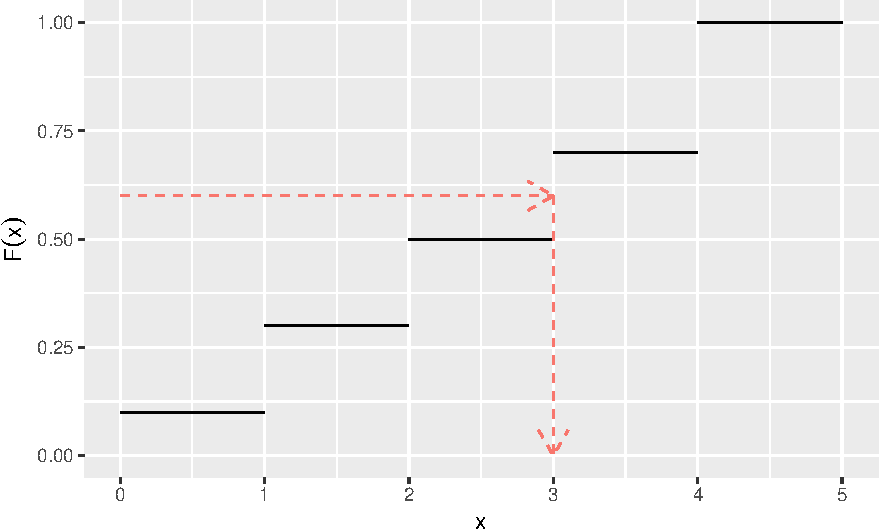
\includegraphics[width=0.7\linewidth]{statistical-computing_files/figure-latex/cdfun-1} 

}

\caption{CDF of the Discrete Random Variable: Illustration for discrete case}\label{fig:cdfun}
\end{figure}

Remembering the algorithm, we can implement \texttt{dplyr::case\_when()}
here.

\begin{Shaded}
\begin{Highlighting}[]
\NormalTok{rcustom <-}\StringTok{ }\ControlFlowTok{function}\NormalTok{(n) \{}
  \KeywordTok{tibble}\NormalTok{(}\DataTypeTok{u =} \KeywordTok{runif}\NormalTok{(n)) }\OperatorTok\StringTok{ }
\StringTok{    }\KeywordTok{mutate}\NormalTok{(}
      \DataTypeTok{x =} \KeywordTok{case_when}\NormalTok{(}
\NormalTok{        u }\OperatorTok{>}\StringTok{ }\DecValTok{0} \OperatorTok{&}\StringTok{ }\NormalTok{u }\OperatorTok{<=}\StringTok{ }\NormalTok{.}\DecValTok{1} \OperatorTok{~}\StringTok{ }\DecValTok{0}\NormalTok{,}
\NormalTok{        u }\OperatorTok{>}\StringTok{ }\NormalTok{.}\DecValTok{1} \OperatorTok{&}\StringTok{ }\NormalTok{u }\OperatorTok{<=}\StringTok{ }\NormalTok{.}\DecValTok{3} \OperatorTok{~}\StringTok{ }\DecValTok{1}\NormalTok{,}
\NormalTok{        u }\OperatorTok{>}\StringTok{ }\NormalTok{.}\DecValTok{3} \OperatorTok{&}\StringTok{ }\NormalTok{u }\OperatorTok{<=}\StringTok{ }\NormalTok{.}\DecValTok{5} \OperatorTok{~}\StringTok{ }\DecValTok{2}\NormalTok{,}
\NormalTok{        u }\OperatorTok{>}\StringTok{ }\NormalTok{.}\DecValTok{5} \OperatorTok{&}\StringTok{ }\NormalTok{u }\OperatorTok{<=}\StringTok{ }\NormalTok{.}\DecValTok{7} \OperatorTok{~}\StringTok{ }\DecValTok{3}\NormalTok{,}
        \OtherTok{TRUE} \OperatorTok{~}\StringTok{ }\DecValTok{4}
\NormalTok{      )}
\NormalTok{    ) }\OperatorTok\StringTok{ }
\StringTok{    }\KeywordTok{select}\NormalTok{(x) }\OperatorTok\StringTok{ }
\StringTok{    }\KeywordTok{pull}\NormalTok{()}
\NormalTok{\}}
\end{Highlighting}
\end{Shaded}

\begin{Shaded}
\begin{Highlighting}[]
\KeywordTok{tibble}\NormalTok{(}
  \DataTypeTok{x =} \KeywordTok{rcustom}\NormalTok{(}\DecValTok{100}\NormalTok{)}
\NormalTok{) }\OperatorTok\StringTok{ }
\StringTok{  }\KeywordTok{ggplot}\NormalTok{(}\KeywordTok{aes}\NormalTok{(}\DataTypeTok{x =}\NormalTok{ x)) }\OperatorTok{+}
\StringTok{  }\KeywordTok{geom_histogram}\NormalTok{(}\KeywordTok{aes}\NormalTok{(}\DataTypeTok{y =}\NormalTok{ ..ndensity..), }\DataTypeTok{binwidth =}\NormalTok{ .}\DecValTok{1}\NormalTok{)}
\end{Highlighting}
\end{Shaded}

\begin{figure}[H]

{\centering 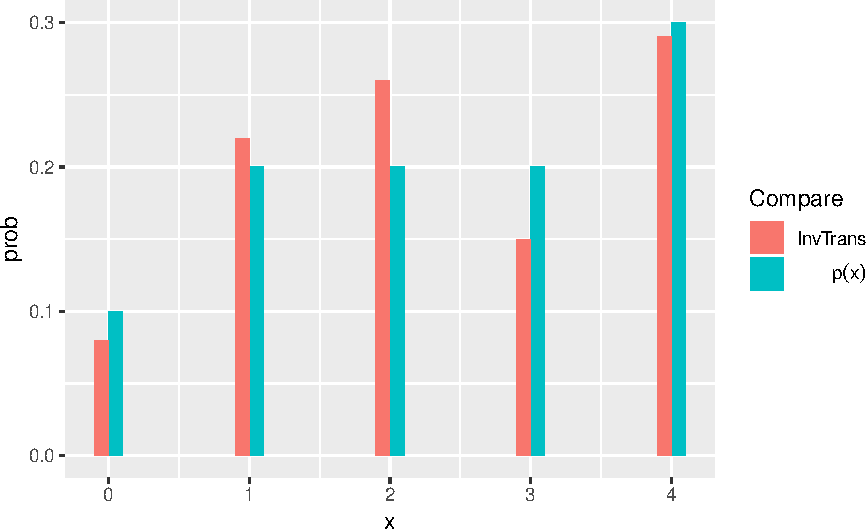
\includegraphics[width=0.7\linewidth]{statistical-computing_files/figure-latex/randmass-1} 

}

\caption{Generated discrete random numbers}\label{fig:randmass}
\end{figure}

See Figure \ref{fig:massfun} and \ref{fig:randmass}. Comparing the two,
the result can be said okay.

\subsection{Problems with inverse
transformation}\label{problems-with-inverse-transformation}

Examples \ref{exm:expon} and \ref{exm:dismass}. We could generate these
random numbers because we aware of

\begin{enumerate}
\def\labelenumi{\arabic{enumi}.}
\tightlist
\item
  analytical \(F_X\)
\item
  \(F^{-1}\)
\end{enumerate}

In practice, however, not all distribution have analytical \(F\).
Numerical computing might be possible, but it is not efficient. There
are other approaches.

\section{The Acceptance-Rejection
Method}\label{the-acceptance-rejection-method}

Acceptance-rejection method does not require analytical form of cdf.
What we need is our \emph{target} density (or mass) function and
\emph{proposal} density (or mass) function. Target function is what we
want to generate. Propsal function is of any random variable that is
\emph{easy to generate random numbers}. From this approach, we can
generate any distribution while computation is not efficient.

\begin{longtable}[]{@{}cc@{}}
\toprule
pdf or pmf & target or proposal\tabularnewline
\midrule
\endhead
\(f\) & target\tabularnewline
\(g\) & proposal - easy to generate random numbers\tabularnewline
\bottomrule
\end{longtable}

First of all, \(g\) should satisfy that

\[spt f \subseteq spt g\]

Next, for some (pre-specified) \(c > 0\)

\[\forall x \in spt f : \frac{f(x)}{g(x)} \le c\]

\subsection{A-R algorithm}\label{a-r-algorithm}

For \(i = 1, \ldots, n\)

\begin{enumerate}
\def\labelenumi{\arabic{enumi}.}
\tightlist
\item
  \(Y \sim g(Y)\)
\item
  \(U \sim unif(0, 1) \perp\!\!\!\perp Y\)
\item
  Accept-Reject step

  \begin{enumerate}
  \def\labelenumii{\alph{enumii}.}
  \tightlist
  \item
    Accept: \(U \le \frac{f(Y)}{cg(Y)} \Rightarrow x_i = Y\)
  \item
    Reject: otherwise, go to step 1
  \end{enumerate}
\end{enumerate}

Collect \(x_1, x_2, \ldots, x_n \stackrel{iid}{\sim} f(x)\).

\subsection{Efficiency}\label{efficiency}

\begin{figure}[H]

{\centering 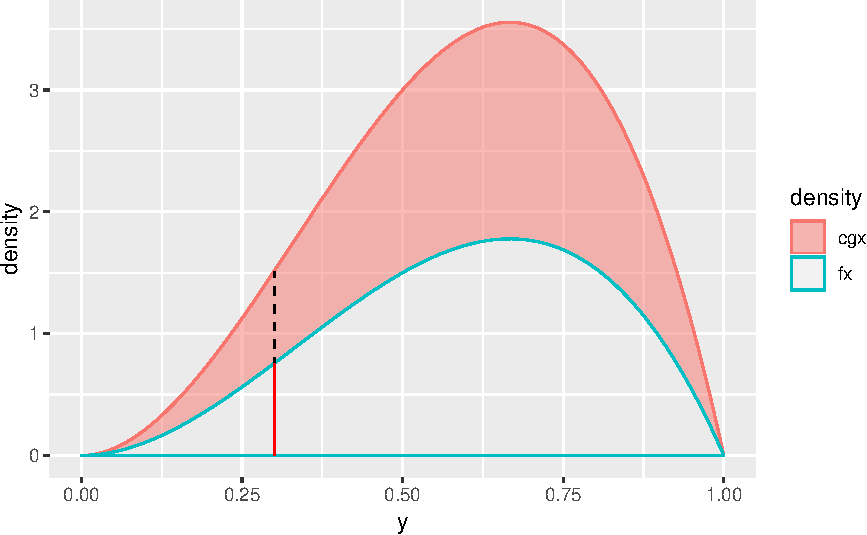
\includegraphics[width=0.7\linewidth]{statistical-computing_files/figure-latex/arprop-1} 

}

\caption{Property of AR method}\label{fig:arprop}
\end{figure}

See Figure \ref{fig:arprop}. This illustrates the motivation of A-R
method. Lower one is \(f(x)\) and the upper one is \(cg(x)\) which
covers \(f\). The algorithm takes random number from \(Y \sim g\) in
each recursive step \(i\), which is represented as a line in the figure.
We can see that

\[0 < \frac{f(x)}{cg(x)} \le 1\]

\chapter{Monte Carlo Integration and Variance Reduction}\label{mcint}

\bibliography{book.bib,packages.bib}


\end{document}
